%\clearpage
\section{Verbindung} \label{sec:connection}

\textbf{Achtung}: Wenn sich mehrere Raspberry Pi Computer im selben Netzwerk befinden, so kann man sich nicht mit dem Hostnamen "
"`raspberrypi.local"' verbinden! In dem Fall muss man die IP-Adresse verwenden oder man �ndert den Hostnamen "`raspberrypi"' auf einen eindeutigen Namen (Datei /etc/hostname). Der GC2-xHAT zeigt die IP-Adresse des Raspberry Pis am Display an.   

\subsection{Linux} 

%\subsection{SSH}

Nach der Einrichtung kann per SSH-Client eine Verbindungen zum Raspberry Pi hergestellt werden. Dazu muss in einem Terminal folgender Befehl eingegeben werden:

\begin{console} 
	ssh -X pi@raspberrypi.local
\end{console}

Um grafische Programme am Host anzeigen zu k�nnen, muss der Parameter \texttt{-X} angegeben werden. "`\textbf{pi}"' ist der Standardbenutzer am System. Dann wird eine X-Server Verbindung via SSH hergestellt. Verbindet man sich zum ersten Mal mit dem Raspberry Pi, so wird noch eine Sicherheitswarnung ausgegeben. Der kryptographische Schl�ssel f�r die Verbindung ist dem lokalen System noch nicht bekannt.%  und muss best�tigt werden.
\begin{screensmall}
The authenticity of host 'raspberrypi.local (192.168.137.10)' can't be established.
ECDSA key fingerprint is SHA256:Dcf3HYgE2GHnNnZ8Xhv8iJ9yA+zvfXBC9COm2eL9i0w.
Are you sure you want to continue connecting (yes/no)? 
Warning: Permanently added 'raspberrypi.local,192.168.137.10' (ECDSA) to the list of known hosts.
\end{screensmall}

Die Frage muss mit \texttt{yes} best�tigt werden. Anschlie�end muss das Default-Passwort von Raspbian "`\textbf{raspberry}"' eingegeben werden. Nun sollte man den Raspberry Pi Prompt \texttt{pi@rasbperrypi:\textasciitilde  \$} sehen. 

Wechselt man zu einem anderen Raspberry Pi mit den gleichen Namen oder installiert das System nochmals, so kann es passieren, dass eine Fehlermeldung ausgegeben wird, weil sich der kryptographische Schl�ssel ge�ndert hat.

\begin{screensmall} 
@@@@@@@@@@@@@@@@@@@@@@@@@@@@@@@@@@@@@@@@@@@@@@@@@@@@@@@@@@@
@    WARNING: REMOTE HOST IDENTIFICATION HAS CHANGED!     @
@@@@@@@@@@@@@@@@@@@@@@@@@@@@@@@@@@@@@@@@@@@@@@@@@@@@@@@@@@@
\end{screensmall} 

%The ECDSA host key for raspberrypi.local has changed,
%and the key for the corresponding IP address 169.254.229.192
%is unknown. This could either mean that
%DNS SPOOFING is happening or the IP address for the host
%and its host key have changed at the same time.
%@@@@@@@@@@@@@@@@@@@@@@@@@@@@@@@@@@@@@@@@@@@@@@@@@@@@@@@@@@@
%@    WARNING: REMOTE HOST IDENTIFICATION HAS CHANGED!     @
%@@@@@@@@@@@@@@@@@@@@@@@@@@@@@@@@@@@@@@@@@@@@@@@@@@@@@@@@@@@
%IT IS POSSIBLE THAT SOMEONE IS DOING SOMETHING NASTY!
%Someone could be eavesdropping on you right now (man-in-the-middle attack)!
%It is also possible that a host key has just been changed.
%The fingerprint for the ECDSA key sent by the remote host is
%SHA256:Dcf2HYyE2GHnNpZ8Xhv8iJ9yj+zvfXBC9COm2eL9i0w.
%Please contact your system administrator.
%Add correct host key in /home/evil/.ssh/known_hosts to get rid of this message.
%Offending ECDSA key in /home/evil/.ssh/known_hosts:9
%remove with:
%ssh-keygen -f "/home/evil/.ssh/known_hosts" -R raspberrypi.local
%ECDSA host key for raspberrypi.local has changed and you have requested strict checking.

In diesem Fall muss man die Verbindung aus den bekannten Hosts l�schen. Hierf�r muss folgendes Kommando ausgef�hrt werden:

\begin{console} 
	ssh-keygen -R raspberrypi.local
\end{console}

Optional kann auch der Parameter \texttt{-o UserKnownHostsFile=/dev/null} beim ssh-Befehl hinzugef�gt werden. Dann erfolgt keine �berpr�fung der Verbindung. 
 \label{sec:connection_ssh}

%\subsubsection{�ber Shell-Script} \label{sec:shellscript}

Am Einfachsten ist es die Verbindung zu Raspberry Pi �ber das vorbereitete PiConnect.sh Shell-Script herzustellen. Es setzt automatisch die Internetweiterleitung und startet die SSH-Verbindung. Es kann vom vorbereitetet Raspbian-Image oder von Github geladen werden.

\begin{console} 
	scp pi@raspberrypi.local:/home/pi/scripts/PiConnect.sh .
\end{console}
oder
\begin{console} 
	wget --trust-server-names https://goo.gl/uwguQo
	sh PiConnect.sh
\end{console}   


\subsection{Windows} \label{sec:connection_windows}

\subsubsection{Xming (X-Server)} \label{sec:connection_xming}

Xming (Download auf \urlsmall{http://www.straightrunning.com/XmingNotes/}) ist ein Programm um einen X-Server unter Windows zur Verf�gung zu stellen. Xming kann mit PuTTY zusammen genutzt werden, um grafische Linux Programme am Windows PC anzeigen und verwenden zu k�nnen. Die Programme laufen dabei auf dem entfernen System, lediglich die Interaktion und grafische Anzeige werden �ber den SSH-Tunnel von Putty �ber Xming verarbeitet.\\
Bei der Auswahl der Komponenten beim Installer sollte man "`Full installtion"' w�hlen. Weiterer Einstellungen bedarf es nicht.

\begin{figure}[ht]
	\centering
	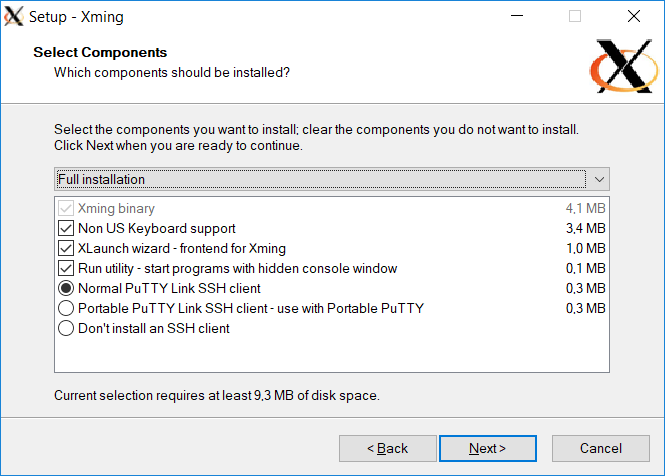
\includegraphics[scale=0.38]{images/Xming_Components.png}
	%	\caption{}
	\label{Putty}
\end{figure}


\subsubsection{PuTTY (SSH-Client)} \label{sec:connection_putty}

PuTTY (Download auf \urlsmall{https://www.chiark.greenend.org.uk/~sgtatham/putty/}) is ein SSH und Telnet Client Programme f�r Windows. Nach der Installation k�nnen die Verbindungen eingerichtet werden.\\
%Zuerst muss bei Terminal/Keyboard "`The Function keys and keypad"' auf Linux gesetzt werden. Dann sollte unter Terminal/Bell die akustische Warnfunktion (Action to happen when a bell occurs) abgeschaltet werden, indem man in den Einstellungen "`None (bell disabled)"' ausw�hlt. Die Zeichenkodierung muss unter Window/Translation auf UTF-8 gesetzt werden. 
Bei Connection/SSH/X11 muss "`Enable X11 forwarding"' eingeschaltet werden. Dann k�nnen auch grafische Programme gestartet werden, wenn ein X-Server am lokalen System verf�gbar ist.\\
Unter Session k�nnen dann die Verbindungsdaten eingegeben werden. Am sichersten ist die Eingabe der IP-Adresse, wenn diese bekannt ist, �blicherweise 192.168.137.10. M�glicherweise ist der Raspberry Pi auch unter dem Hostnamen raspberrypi.local erreichbar. Bei "`connection type"' gibt man SSH mit Port 22 an.\\
Bei "`Saved Sessions"' kann ein beliebiger Name wie z.~B. "`192.168.137.10 - Raspberry Pi"' eingetragen werden. Mit der Schaltfl�che "`Save"' werden nun alle Einstellungen unter diesem Namen gespeichert. Mit der Schaltfl�che "`Load"' k�nnen die Einstellungen wieder geladen werden. Nach dem Dr�cken der Schaltfl�che "`Open"' wird die Verbindung aufgebaut und man kann sich mit dem Benutzernamen "`\textbf{pi}"' und dem Passwort "`\textbf{raspberry}"' anmelden.\\


\begin{figure}[ht]
	\centering
	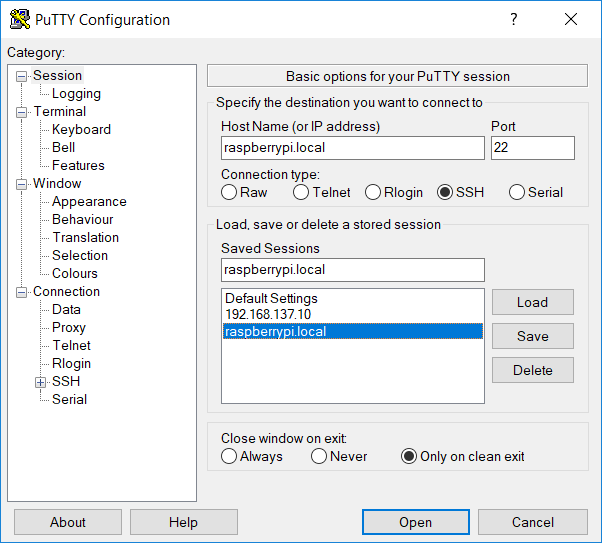
\includegraphics[scale=0.295]{images/Putty-Session-Raspjamming.png}
	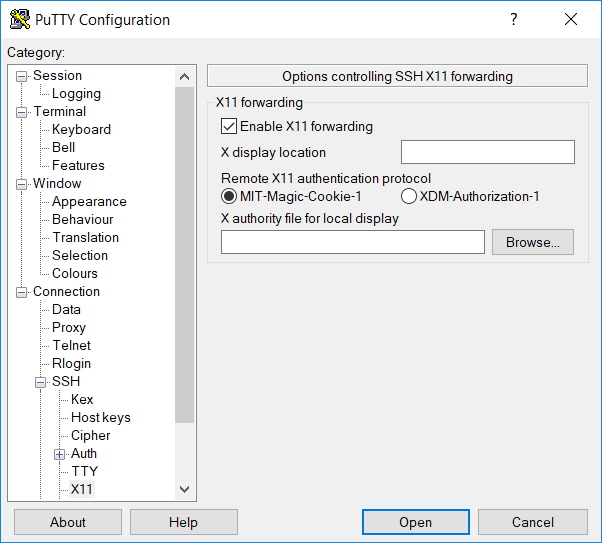
\includegraphics[scale=0.49]{images/Putty-X11.png}
	%	\caption{}
	\label{Putty}
\end{figure}
